\documentclass[11pt]{beamer}

\mode<presentation>
{
\usetheme{Warsaw}
}

\usepackage{amsbsy,amssymb}
\usepackage{amsmath}
\usepackage{graphicx}
\usepackage[compatibility=false,font=scriptsize]{caption}
\usepackage[font=scriptsize]{subcaption}
\usepackage{booktabs}

\usepackage{paralist}
\newenvironment{innerlist}[1][\enskip\textbullet]%
        {\begin{compactenum}[#1]}{\end{compactenum}}


%% ---------------------------------------------------------------- %%
%% ---------------------------------------------------------------- %%

\title{The U.S. Presidential Race}
\subtitle{Comparing Coverage Across Three Major Sources}
\author{Thomas Brawner}
\institute{\normalsize Galvanize, Inc.}
\date{September 2015}

%% ---------------------------------------------------------------- %%
%% ---------------------------------------------------------------- %%

\begin{document}
\maketitle

%% ---------------------------------------------------------------- %%
%% ---------------------------------------------------------------- %%

\begin{frame}
\frametitle{Two objectives}

\vspace{5mm}

\begin{itemize}
	\item {\it Is there a difference in coverage?} 
	\vspace{3mm}
	\begin{itemize}
		\item[$\rightarrow$] Classification Problem
	\end{itemize}
	\vspace{6mm}
	\item {\it What is the difference?}
	\vspace{3mm}
	\begin{itemize}
		\item[$\rightarrow$] Topic Modeling 
		\vspace{2mm}
		\item[$\rightarrow$] Sentiment Analysis 
	\end{itemize}
\end{itemize}

\end{frame}

%% ---------------------------------------------------------------- %%
%% ---------------------------------------------------------------- %%

\begin{frame}
\frametitle{Data collection}

\vspace{5mm}

\begin{innerlist}
	\item[$\sharp~$] Scrape {\it Guardian}, {\it New York Times}, {\it Wall Street Journal}
	\vspace{4mm}
	\item[$\sharp~$] January to August 2015
	\vspace{4mm}
	\item[$\sharp~$] Raw data $\rightarrow$ MongoDB
	\vspace{4mm}
	\item[$\sharp~$] Filter on candidates
	\vspace{4mm}
	\item[$\sharp~$] TF-IDF, 2000 terms
\end{innerlist}

\end{frame}

%% ---------------------------------------------------------------- %%
%% ---------------------------------------------------------------- %%

\begin{frame}
\frametitle{Multiclass classification accuracy}

\begin{table}
\centering
\scriptsize 
\begin{tabular}{lcccc}
\toprule
				& Global		& Guardian 	& New York Times	& Wall Street Journal	\\ 
\midrule
Naive Bayes 		& 0.703		& 0.414		& 0.965	 		& 0.340				\\
Random Forest		& 0.905		& 0.783		& 0.998			& 0.809 				\\ 
Gradient Boosting	& 0.921		& 0.856		& 0.983			& 0.833				\\ 
$N$				& 3757    		& 1018		& 2087 			& 652	 			\\
\bottomrule
\end{tabular}
\end{table}

\end{frame}

%% ---------------------------------------------------------------- %%
%% ---------------------------------------------------------------- %%

\begin{frame}
\frametitle{Topic modeling strategy}

\[
\begin{bmatrix}
        		v_{11} & \cdots & v_{1t} & \cdots & v_{1T} \\
		\vdots & \ddots & \vdots & \ddots & \vdots\\
		v_{i1} & \cdots & v_{it} & \cdots & v_{iT} \\
        		\vdots & \ddots & \vdots & \ddots & \vdots\\
        		v_{N1} & \cdots & v_{Nt} & \cdots & v_{NT}
\end{bmatrix}
=
\]

\[
\begin{bmatrix}
        		w_{11} & \cdots & w_{1K} \\
		\vdots & \ddots & \vdots \\
		w_{i1} & \cdots & w_{iK} \\
        		\vdots & \ddots & \vdots\\
        		w_{N1} & \cdots & w_{NK}
\end{bmatrix}
\times 
\begin{bmatrix}
        		h_{11} & \cdots & h_{1t} & \cdots & h_{1T} \\
		\vdots & \ddots & \vdots & \ddots & \vdots\\
		h_{K1} & \cdots & h_{Kt} & \cdots & h_{KT} \\
\end{bmatrix}
\]

\end{frame}

%% ---------------------------------------------------------------- %%
%% ---------------------------------------------------------------- %%

\begin{frame}
\frametitle{Topic modeling strategy (cont.)}


\vspace{5mm}

\begin{itemize}
	\item With $\mathbf{H}_{K \times T}$
	\vspace{2mm}
	\begin{innerlist}
		\item sort descending for each $k$ 
		\item top 50 terms $\rightarrow$ Word Cloud
	\end{innerlist}
	\vspace{6mm}
	\item With $\mathbf{W}_{N \times K}$
	\vspace{2mm}
	\begin{innerlist}
		\item group by source, month $\rightarrow$ time series
		\item group by source  $\rightarrow$ bar plots
	\end{innerlist}
\end{itemize}


\end{frame}


%% ---------------------------------------------------------------- %%
%% ---------------------------------------------------------------- %%

\begin{frame}
\frametitle{Hillary's Email}

\begin{figure}
\centering
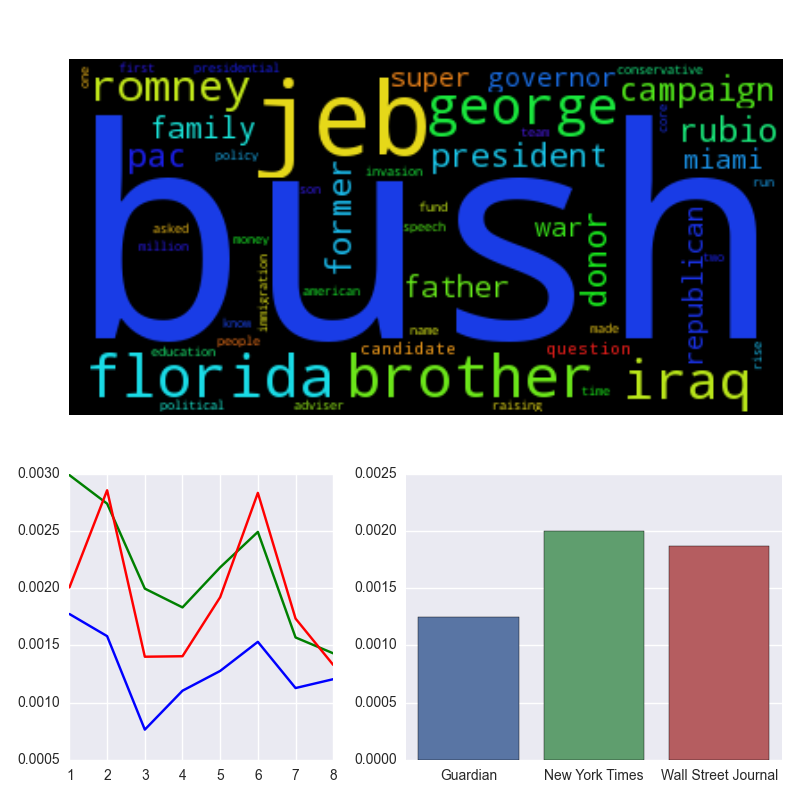
\includegraphics[width=85mm,height=75mm]{figures/source_topic2.png}
\end{figure} 

\end{frame}

%% ---------------------------------------------------------------- %%
%% ---------------------------------------------------------------- %%

\begin{frame}
\frametitle{Chris Christie}

\begin{figure}
\centering
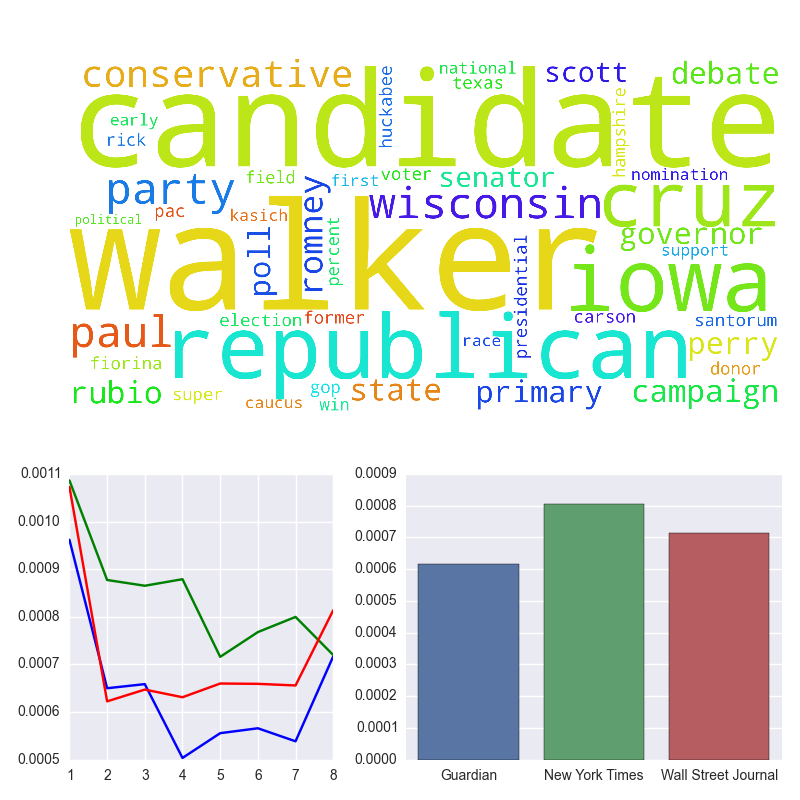
\includegraphics[width=85mm,height=75mm]{figures/source_topic0.png}
\end{figure} 

\end{frame}

%% ---------------------------------------------------------------- %%
%% ---------------------------------------------------------------- %%

\begin{frame}
\frametitle{The Rise of Trump}

\begin{figure}
\centering
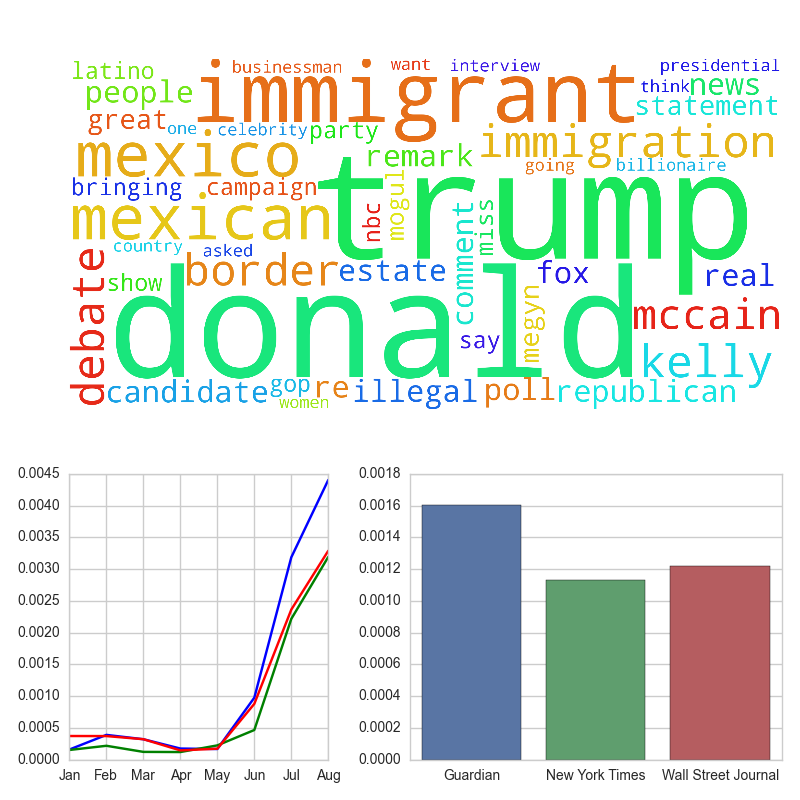
\includegraphics[width=85mm,height=75mm]{figures/source_topic10.png}
\end{figure} 

\end{frame}

%% ---------------------------------------------------------------- %%
%% ---------------------------------------------------------------- %%

\begin{frame}
\frametitle{Gun Violence}

\begin{figure}
\centering
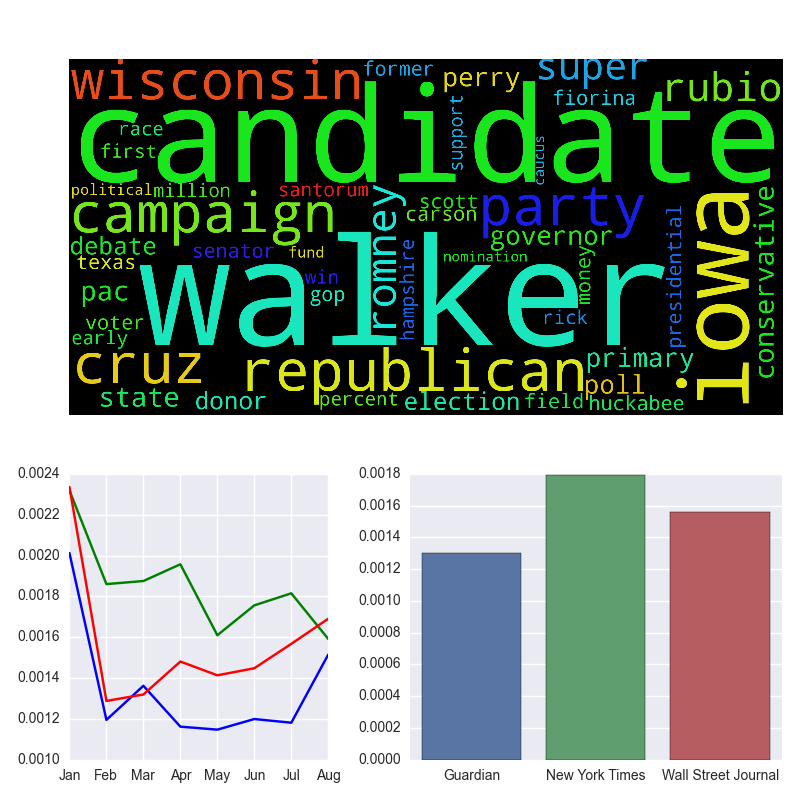
\includegraphics[width=85mm,height=75mm]{figures/source_topic1.png}
\end{figure} 

\end{frame}

%%
%%

\begin{frame}
\frametitle{Gun Violence by Outlet}

\begin{figure}
\centering
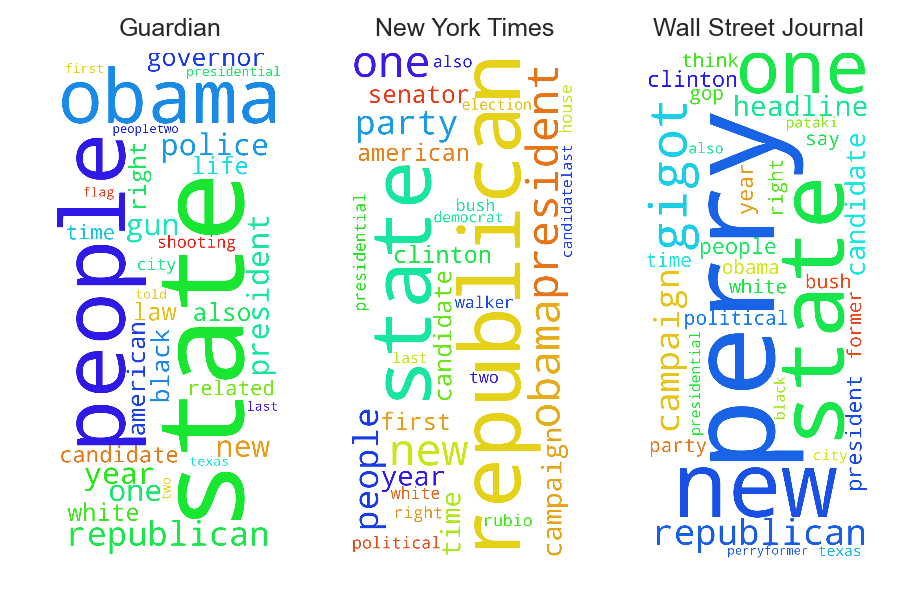
\includegraphics[width=100mm,height=75mm]{figures/source_within_topic1.png}
\end{figure} 

\end{frame}

%%
%%

\begin{frame}
\frametitle{Gun Violence by Outlet}

\begin{figure}
\centering
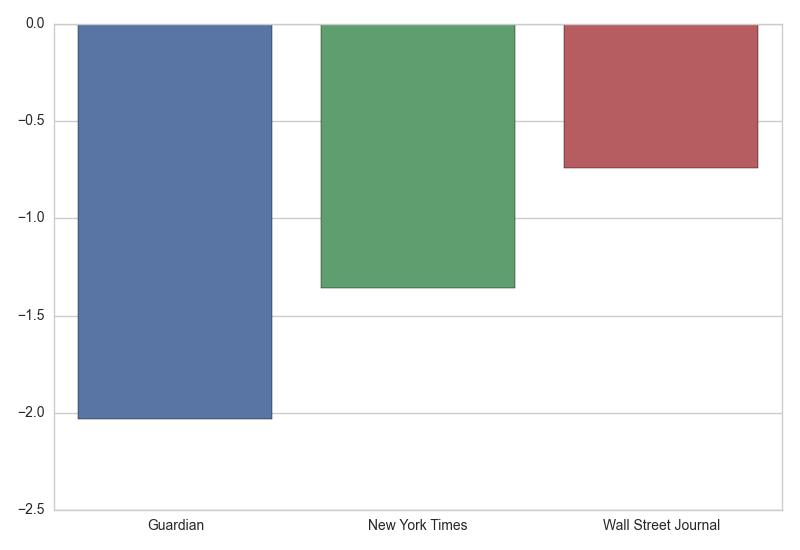
\includegraphics[width=100mm,height=75mm]{figures/source_sentiment_topic1.png}
\end{figure} 

\end{frame}

%% ---------------------------------------------------------------- %%
%% ---------------------------------------------------------------- %%

\begin{frame}
\frametitle{Gay Marriage}

\begin{figure}
\centering
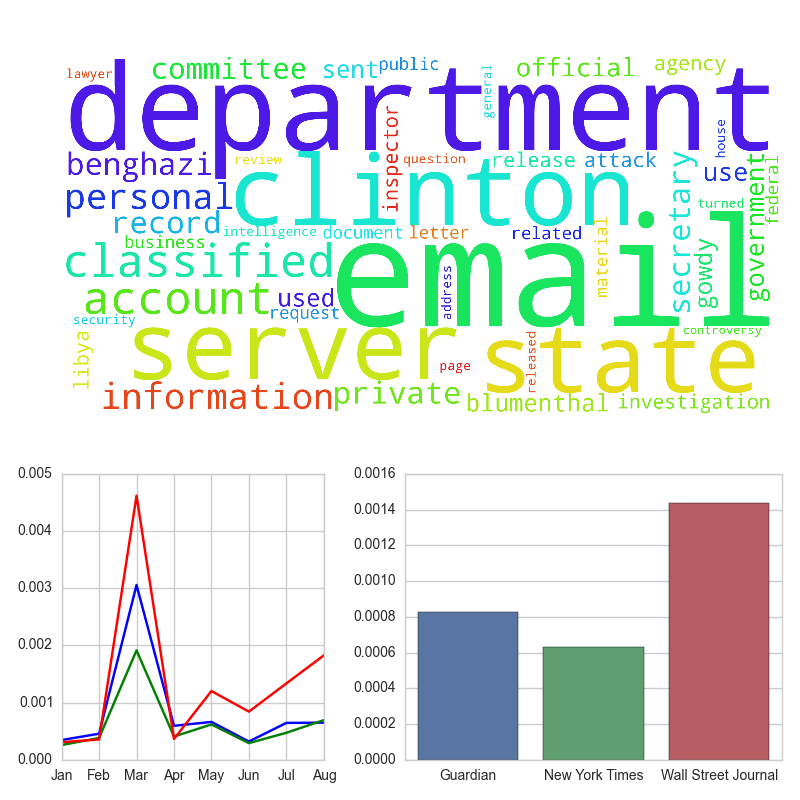
\includegraphics[width=85mm,height=75mm]{figures/source_topic14.png}
\end{figure} 

\end{frame}

%%
%%

\begin{frame}
\frametitle{Gay Marriage by Outlet}

\begin{figure}
\centering
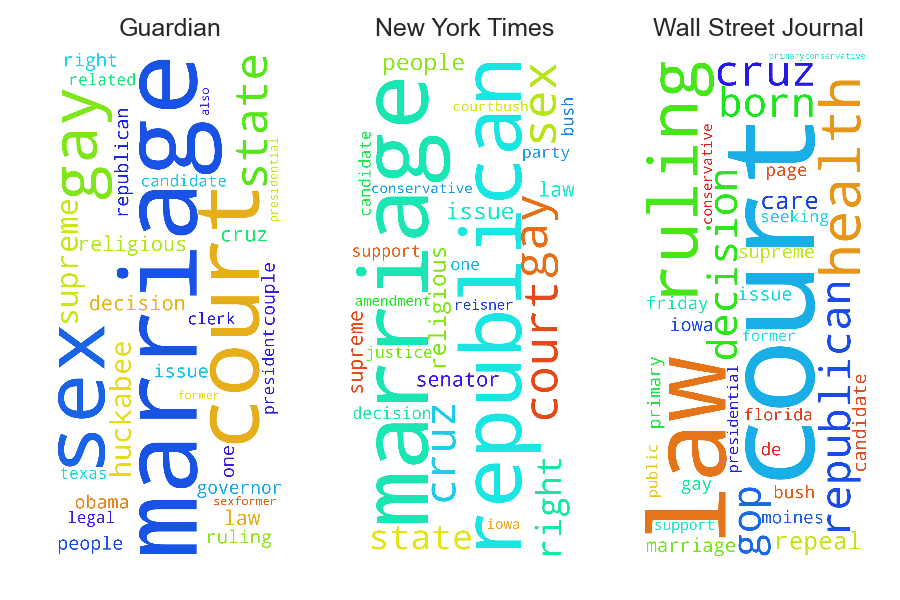
\includegraphics[width=100mm,height=75mm]{figures/source_within_topic14.png}
\end{figure} 

\end{frame}

%%
%%

\begin{frame}
\frametitle{Gay Marriage Sentiment by Outlet}

\begin{figure}
\centering
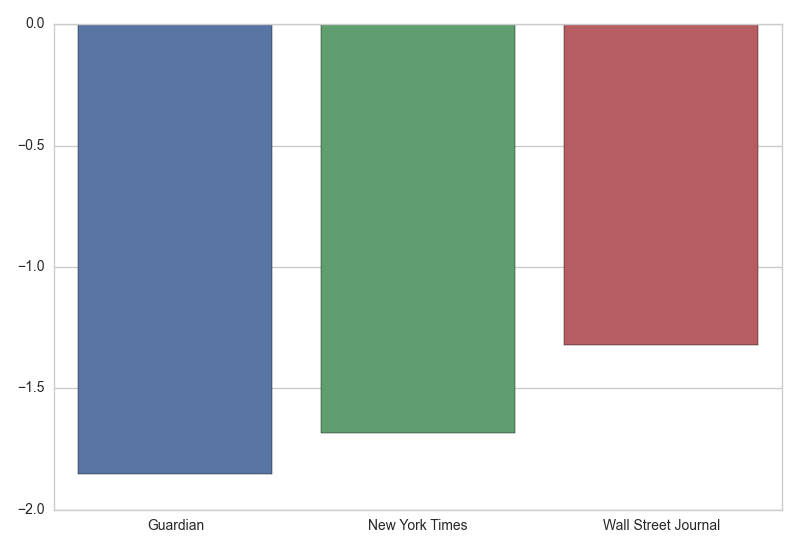
\includegraphics[width=100mm,height=75mm]{figures/source_sentiment_topic14.png}
\end{figure} 

\end{frame}

%% ---------------------------------------------------------------- %%
%% ---------------------------------------------------------------- %%

\begin{frame}
\frametitle{Iran Nuclear Deal}

\begin{figure}
\centering
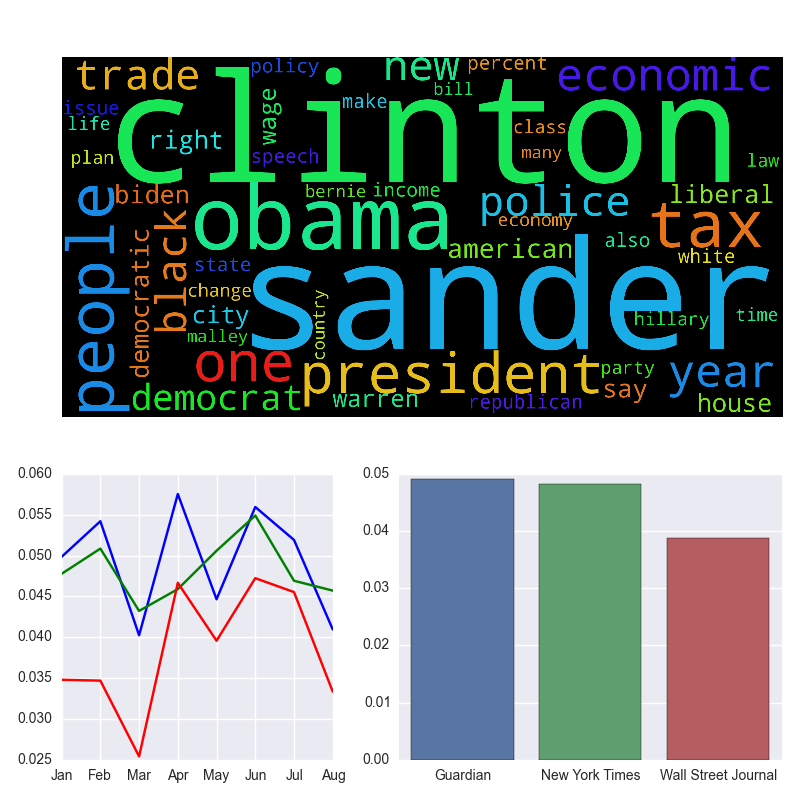
\includegraphics[width=85mm,height=75mm]{figures/source_topic3.png}
\end{figure} 

\end{frame}

%%
%%

\begin{frame}
\frametitle{Iran Nuclear Deal by Outlet}

\begin{figure}
\centering
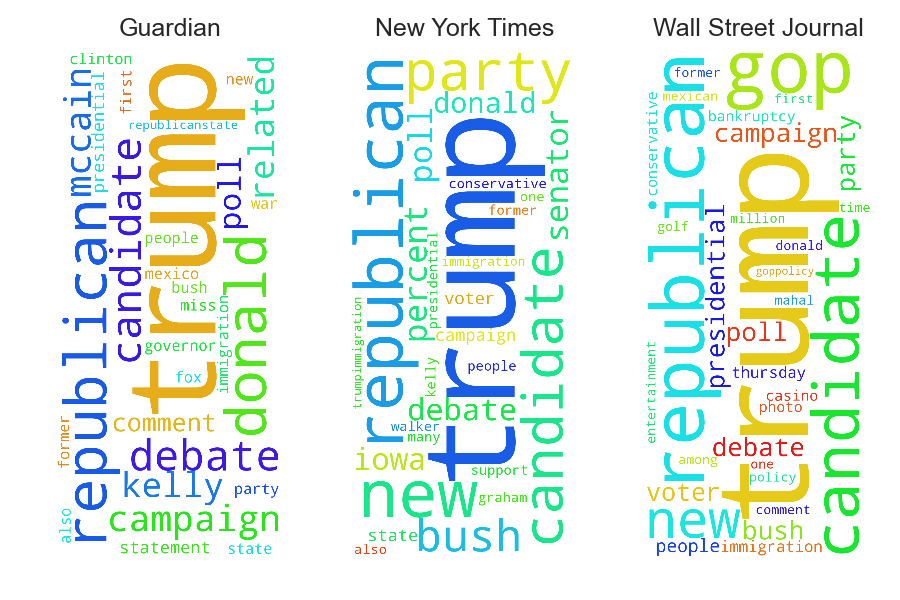
\includegraphics[width=100mm,height=75mm]{figures/source_within_topic3.png}
\end{figure} 

\end{frame}

%%
%%

\begin{frame}
\frametitle{Iran Nuclear Deal by Outlet}

\begin{figure}
\centering
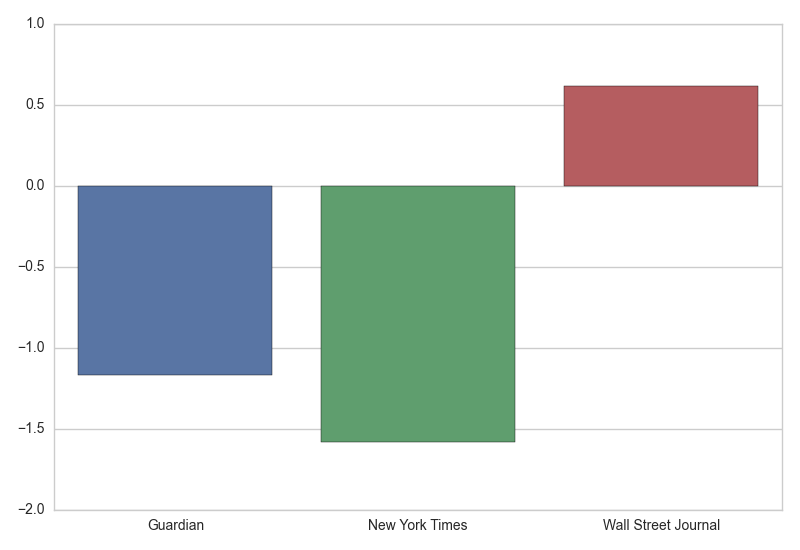
\includegraphics[width=100mm,height=75mm]{figures/source_sentiment_topic3.png}
\end{figure} 

\end{frame}

%% ---------------------------------------------------------------- %%
%% ---------------------------------------------------------------- %%

\begin{frame}
\frametitle{Next steps}

\vspace{5mm}

\begin{innerlist}
	\item[$\sharp~$] More data: collect through duration of election
	\vspace{4mm}
	\item[$\sharp~$] More data: {\it Washington Post}, {\it Financial Times}, etc.
	\vspace{4mm}
	\item[$\sharp~$] Finer classification model tuning 
	\vspace{4mm}
	\item[$\sharp~$] What are we misclassifying? 
\end{innerlist}

\end{frame}

%% ---------------------------------------------------------------- %%
%% ---------------------------------------------------------------- %%

\end{document}

%% ---------------------------------------------------------------- %%
%% ---------------------------------------------------------------- %%